\section{Esercizio 27}
\textit{\textbf{Descrizione:}  Scrivere le function ausiliarie, per la function del precedente esercizio, che implementano i metodi iterativi di Jacobi e Gauss-Seidel.}\newline
\emph{Soluzione: }\\~\\
\textbf{il metodo di Jacobi:}
\\~\\
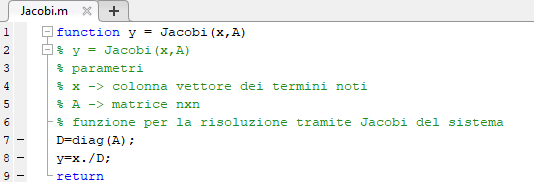
\includegraphics[width=1.3\linewidth]{img/Jacobi}\\~\\
\textbf{il metodo di GaussSeidel:}
\\~\\
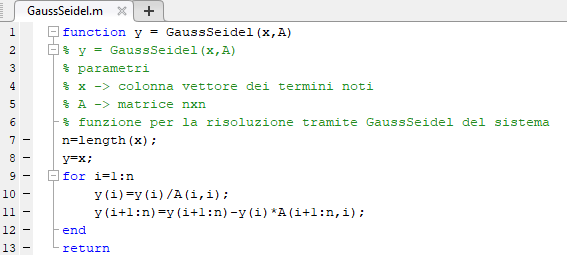
\includegraphics[width=1.3\linewidth]{img/GS}\newpage